%%=============================================================================
%% Methodologie
%%=============================================================================

\chapter{\IfLanguageName{dutch}{Methodologie}{Methodology}}
\label{ch:methodologie}

%% : Hoe ben je te werk gegaan? Verdeel je onderzoek in grote fasen, en
%% licht in elke fase toe welke stappen je gevolgd hebt. Verantwoord waarom je
%% op deze manier te werk gegaan bent. Je moet kunnen aantonen dat je de best
%% mogelijke manier toegepast hebt om een antwoord te vinden op de
%% onderzoeksvraag.

Na het literatuuronderzoek is het doel van deze bachelorproef om een website te ontwikkelen waarmee \textit{elderspeak} kan gedetecteerd worden via een detector. In het literatuurgedeelte werd ook theoretisch beschreven wat AI is en welke types er zijn, wat en hoe \textit{natural language processing} werkt en hoe men achtergrondlawaai filtert.

Alle eigenschappen van \textit{elderspeak} worden herkend a.d.h.v.\ Python-bibliotheken en niet op basis van een zelfgemaakt AI-model. Men moet immers het warm water nieuw opnieuw uitvinden. Zo stelde \textcite{Beeckman2021} het volgende: ``Deze bachelorproef heeft geen meerwaarde kunnen aantonen voor het gebruik van een CNN. Wegens omstandigheden was het niet mogelijk te beschikken over een grote dataset wat leidt tot slechte voorspellingen van het model. Het model voorspelt een classificatie aan dezelfde accuraatheid dan dat gokken zou teweegbrengen. Dit maakt het huidige model onbruikbaar in de praktijk.''. De denkpiste om zelf een AI-model te maken, werd door deze stelling snel ontkracht. Ook de promotor Van Boven haalde aan dat er genoeg Python-bibliotheken ter beschikking zijn om de opdracht op die manier tot een goed einde te brengen.

Sommige methoden konden gekopieerd worden van de bijlagen van de studenten die hiervoor aan dit project gewerkt hebben, maar niet alle code stond beschreven in die bijlage. Daarnaast had \textcite{Standaert2021} geen GitHub-\textit{repository}, waardoor de code niet snel kon hergebruikt worden. Ook zaten er af en toe kleine foutjes in de code waarbij het nodig was om die op te lossen. Om die reden zal er in Hoofdstuk~\ref{ch:vervolg} een deeltje aan bod komen over belang van het delen van code.

\section{Berekeningen in back-end}
Deze voorbeeldapplicatie, geschreven in Python en gebruikmakend van het \textit{micro-framework} Flask, is een webapplicatie die verschillende webpagina's bevat. De code van de volledige Flask-applicatie is te vinden in bijlage~\ref{bijlage:flask}. Naast de inleidende pagina, zie figuur~\ref{fig:home_page}, bevat deze ook een detector. Voor het begin zie figuur~\ref{fig:detector_begin_page}, en na het analyseren ziet de webpagina er als volgt uit, zie figuur~\ref{fig:detector_end_page}. Er kan ook bestudeerd worden wat \textit{secondary baby talk} is in de vorm van een oplijsting, zie figuur~\ref{fig:eigenschappen_page}. Op die manier kan iedereen, maar specifiek studenten in de zorg, actief en passief leren wat \textit{elderspeak} precies is. Enerzijds kunnen ze de eigenschappen leren herkennen door zelf actief stukjes spraak op te nemen. Die worden dan geanalyseerd zodat men kan zien welke eigenschappen er aanwezig waren. Anderzijds kunnen ze passief leren wat de eigenschappen zijn van \textit{elderspeak} en hoe men dat kan voorkomen.

De applicatie bestaat uit twee onderdelen. Eerst wordt een afbeelding van twee jonge vrouwen getoond, dit is een foto van HOGENT voor copyrightrechten. Er wordt dan gevraagd om tegen hen te spreken en audio op te nemen. Dat fragment wordt dan geanalyseerd voor de eigenschappen van toonhoogte en stemvolume, wat gebruikt kan worden als vergelijkingsmateriaal voor het volgende fragment.
Vervolgens wordt er een foto van een oudere vrouw getoond waarbij er gevraagd wordt om haar aan te spreken. Na dit tweede fragment worden de aanwezige \textit{elderspeak}-eigenschappen weergegeven. Ook indien er geen kenmerken aanwezig waren, wordt dit getoond op de website.


\begin{figure}
    \centering
    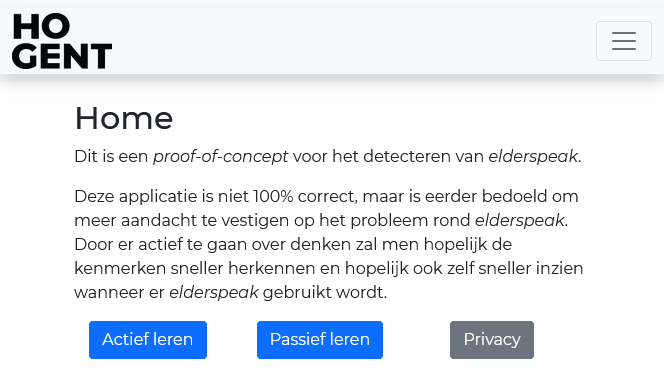
\includegraphics[width=1\textwidth]{./img/home_website}
    \caption{\label{fig:home_page} Home pagina website}
\end{figure}


\begin{figure}
    \centering
    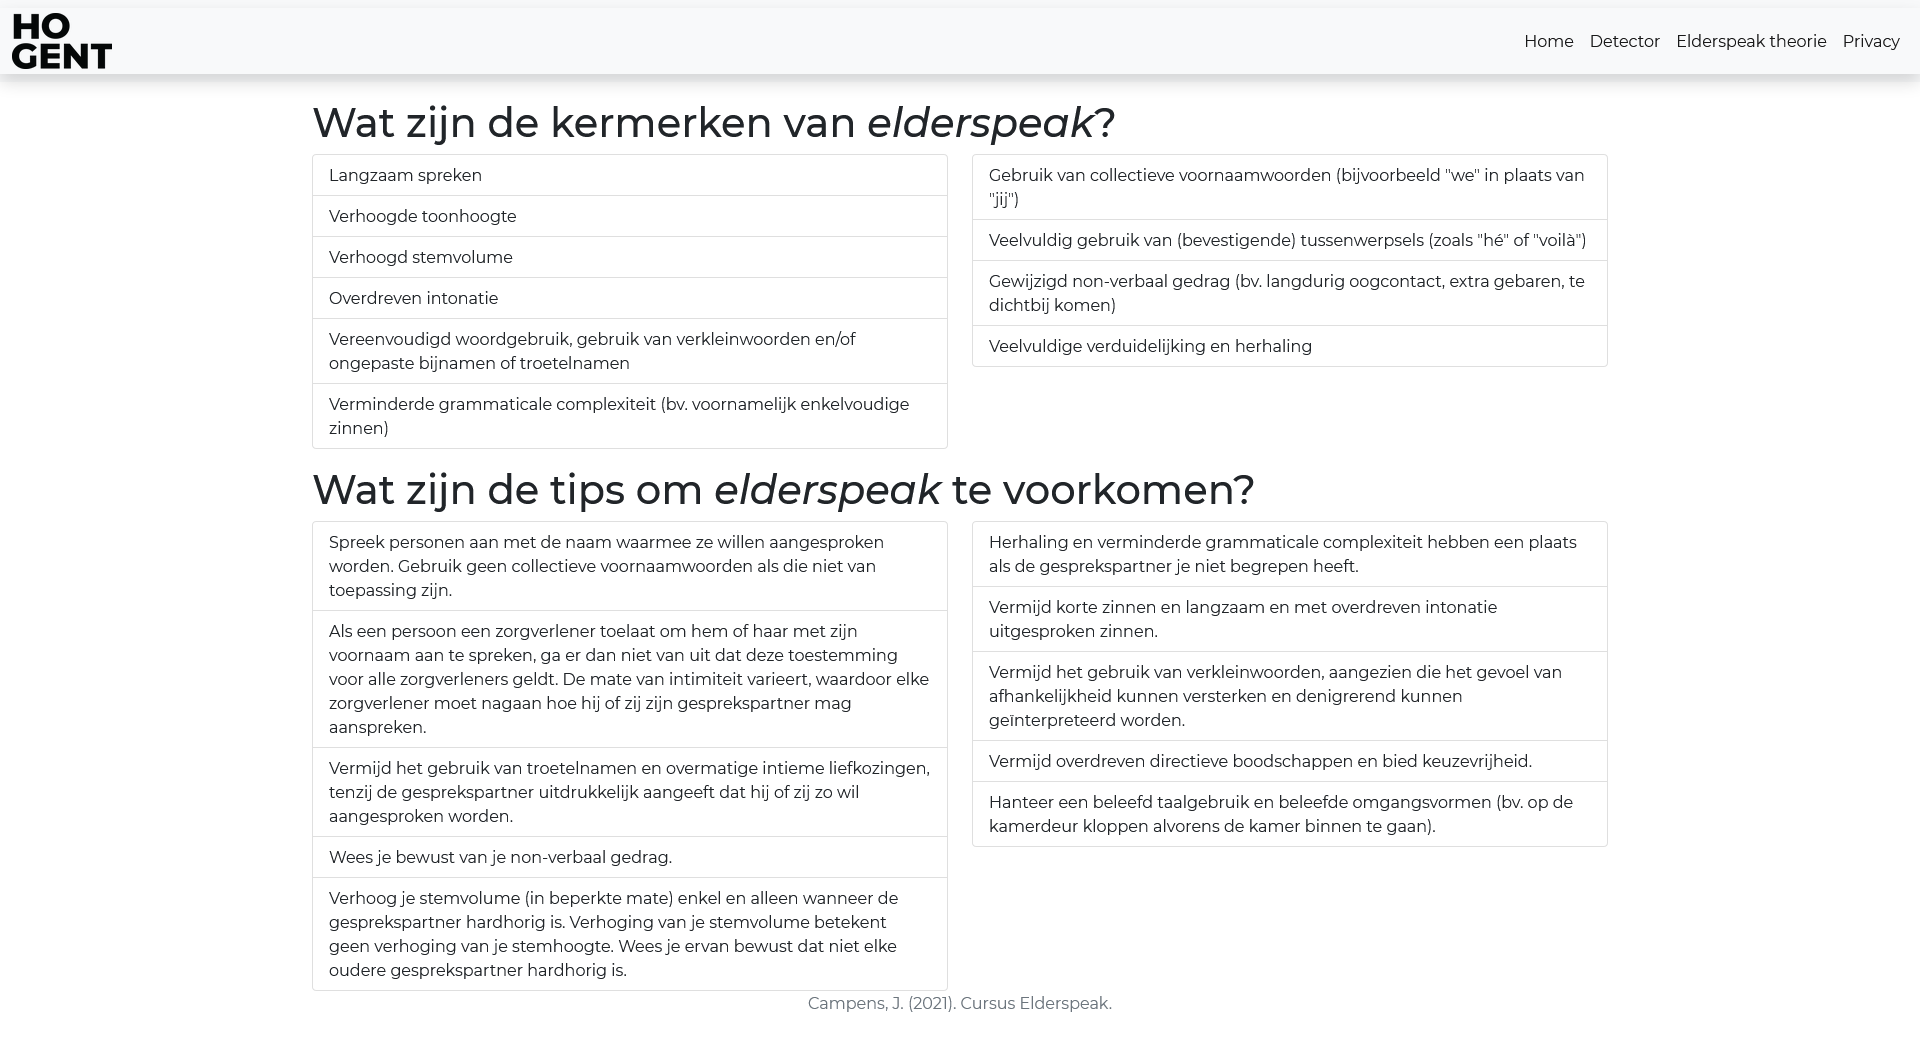
\includegraphics[width=1\textwidth]{./img/eigenschappen_elderspeak_website}
    \caption{\label{fig:eigenschappen_page} Eigenschappen \textit{elderspeak} op de website.}
\end{figure}

\begin{figure}
    \centering
    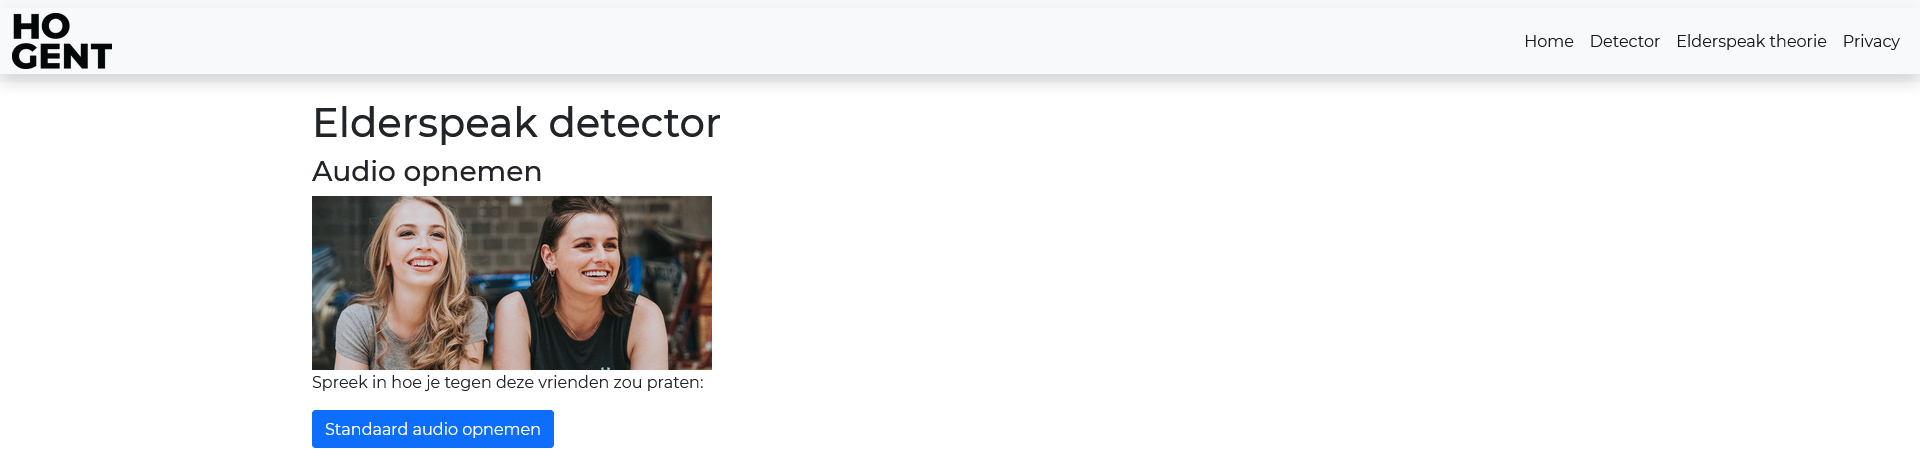
\includegraphics[width=1\textwidth]{./img/detector_begin_elderspeak}
    \caption{\label{fig:detector_begin_page} Detector bij het begin.}
\end{figure}

\begin{figure}
    \centering
    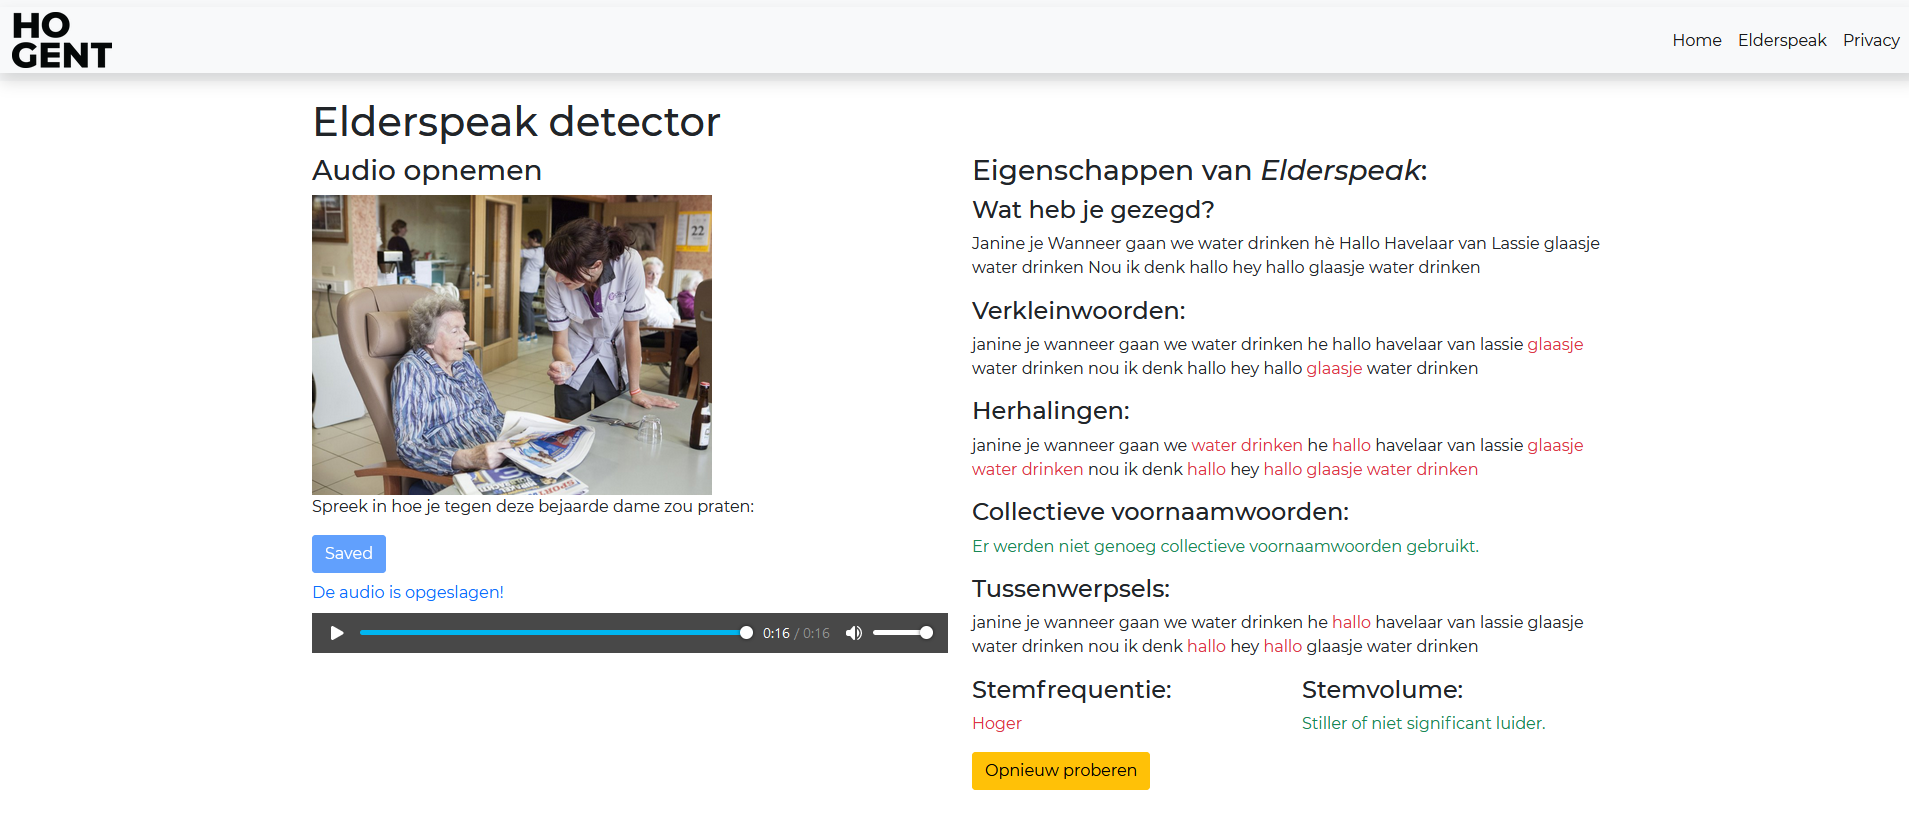
\includegraphics[width=1\textwidth]{./img/dector_na_detecteren}
    \caption{\label{fig:detector_end_page} Detector na het analyseren.}
\end{figure}


\subsection{Speech recognition}
De basis van de applicatie is het herkennen van de spraak die wordt opgenomen op de website. Uiteraard moet dit niet van nul opgebouwd worden, maar kan er gebruikgemaakt worden van een bestaande Python-bibliotheek. \textcite{Standaert2021} bemerkte in zijn bachelorproef dat  de Google Speech Recognition-API de beste optie is om te gebruiken, omdat deze het beste presteert. Hij vatte dit samen in zijn conclusie: ``Uit verschillende onderzoeken of studies waar men verschillende ASR-systemen met elkaar vergeleken [\textit{sic}] kwam de Google Speech-API er altijd als beste uit. En dit in alle aspecten.''. Daarnaast gebruikt de Google Speech-API ook \textit{natural language processing} of NLP om beter te kunnen begrijpen wat er precies gezegd werd~\autocite{GoogleCloud2022}. Hoe dit precies werkt, is na te lezen in het literatuuronderzoek, namelijk in Hoofdstuk~\ref{ch:stand-van-zaken}.

Bij de spraakherkenning kwam er wel een groot probleem aan het licht. De Google \textit{Speech Recognition}-API kan alleen overweg met \textit{wav}- en \textit{flac}-bestanden én kan maar een bepaalde periode, ongeveer 2 tot 3 minuten, gratis herkennen. Het probleem is dat de audio gecapteerd werd in een \textit{mp3}-formaat. Het was dus noodzakelijk om eerst een conversie te maken van \textit{mp3} naar \textit{flac}, en om het audiobestand op te delen in deelbestandjes of \textit{chuncks}, zodat er geen betalende versie voor nodig was. De gebruikte technologie hierbij was ``ffmpeg''. Hierbij was het nodig dat de lengte van het bestand berekend werd, in hoeveel \texit{chunks} het bestand opgedeeld moet worden a.d.h.v.\ de limiet die de gratis Google \textit{Speech Recognition}-API toeliet. Hoe de conversie heel precies gebeurt, is gedetailleerd te vinden in bijlage~\ref{bijlage:speech_recognition}.

Het gebruiken van die API is relatief gemakkelijk. Een extra optie is dan ook ter beschikking om achtergrondlawaai een beetje weg te filteren. Door de optie \newline`ajust\_for\_ambient\_noice(source)' aan te zetten, zal de bibliotheek zich aanpassen aan de geluidsbron om de klanken beter op te nemen alvorens die worden doorgestuurd naar de spraakherkenning-API. Deze methode gebruikt de techniek die beschreven is in het literatuuronderzoek over achtergrondlawaai.

Eens dit ingesteld is, worden de audiobestanden meegegeven en krijgt het systeem de tekst terug waarvan het AI-model van Google de tekst herkend heeft. Uiteraard werkt dit niet feilloos, maar  het functioneert behoorlijk goed voor een gratis versie. Dit vormt de basis voor de volgende methoden. Die zijn te vinden in de tussentitels hieronder:

\subsection{Verkleinwoorden}
Om verkleinwoorden te herkennen werd de methode van \textcite{Standaert2021} gehanteerd. Daarbij wordt er gekeken of woorden langer zijn dan 3 letters en ze niet voorkomen in de lijst die geen verkleinwoorden zijn. Enkele voorbeelden die wel eindigen op ``-je'', ``-ke'', ``-kes'' of ``-jes'', maar geen verkleinwoorden zijn, zijn: poffertje, meisje, koopje, etentje, dutje, toetje, mannelijke, vrouwelijke etc. Extra woorden die geen verkleinwoorden zijn, heeft \textcite{Standaert2021} in zijn project gedefinieerd. Daarover schrijft hij het volgende:
``Na verder onderzoek en testen blijkt dat er nog een hoop andere woorden zijn die eindigen
op -ke. Namelijk bijna alle bijvoeglijke naamwoorden. Denk maar aan ’sterke’ of ’leuke’.
Maar omdat er niet direct een onderscheid te maken valt tussen bijvoeglijke naamwoorden
die eindigen op -ke of verkleinwoorden die eindigen op -ke zal er gecontroleerd worden op
alle andere woorden die eindigen op een -ke maar geen verkleinwoord zijn door een lijst
van deze woorden te includeren in de applicatie. Deze komt van enyclopedy.nl(Encylo.nl,
2021). In deze lijst zijn ook alle steden, gemeenten en deelgemeenten gestoken die eindigen
op -ke, simpelweg door een lijst te trekken van alle steden, gemeenten en deelgemeenten
en te gaan kijken welke er eindigen op -ke. Want bijvoorbeeld de gemeente Merelbeke
eindigt op -ke maar zou ook niet als verkleinwoord aanschouwd mogen worden. De lijst
bestaat dus uit alle bijvoeglijke naamwoorden die eindigen op -ke, alle gemeentes die
eindigen op -ke én ook nog een aantal uitzonderingen. Zoals ’ter zake’ of ’ter sprake’.''~\autocite{Standaert2021}. Dus alle casusen die hierboven beschreven staan, zijn dan ook opgeslagen in de applicatie. Hierdoor zullen deze woorden niet geklasseerd worden als verkleinwoord.

Wanneer een woord eindigt op ``-je'', ``-ke'', ``-kes'' of ``-jes'' én niet op de bovenstaande lijst staan, wordt deze dan bijgehouden in een lijst. Op het einde wordt ofwel bepaald dat er geen verkleinwoorden aanwezig waren, of worden alle verkleinwoorden in de tekst in het rood aangeduid. De code voor deze methode kan gevonden worden in bijlage~\ref{bijlage:verkleinwoorden}.

\subsection{Herhalingen}
Om herhalingen te herkennen werd er eveneens gebruik gemaakt van de methode die \textcite{Standaert2021} beschreven heeft. Daarbij worden de voorbije 25 woorden bijgehouden waarin eventuele herhalingen bewaard worden in een lijst.
Die zullen later gebruikt worden om een mooie weergave te maken van de aanwezige herhalingen.
De code om herhalingen te detecteren is te vinden in bijlage~\ref{bijlage:herhalingen}.

\subsection{Collectieve voornaamwoorden}
Een voorbeeld van een collectief voornaamwoord is het gebruiken van ``we'' / ``wij''.Volgende zinnen verduidelijken dit voorbeeld: ``Gaan we onze patatjes opeten?'', ``Kunnen we alleen naar de wc?'', ``Awel, wat zijn we aan het doen?''.

Er wordt bijgehouden hoeveel keer er collectieve voornaamwoorden gebruikt worden in de tekst. Als een woord meer dan één keer voorkomt, dan zal de applicatie dit weergeven. Dit is zo ingesteld omdat het niet mag worden weergegeven wanneer er iemand eenmalig het woord ``we'' gebruikt.
Wanneer er geen of minder dan twee collectieve voornaamwoorden gebruikt worden, zal de applicatie zeggen dat er geen of niet genoeg aanwezig waren om als \textit{elderspeak} vast te stellen.

Natuurlijk duiden twee of meer collectieve voornaamwoorden niet direct op \textit{elderspeak}, maar het geeft wel al een richting. De persoon in kwestie moet natuurlijk de theorie over \textit{elderspeak} kennen en moet daarna ook kritisch zijn over het resultaat, onder meer met behulp van een zelfreflectie.

\subsection{Tussenwerpsels}
Het veelvuldig gebruik van tussenwerpsels is een eigenschap van \textit{elderspeak} en ook dit wordt herkend. Enkele voorbeelden van tussenwerpsels die herkend worden zijn: ``oh'', ``oeps'', ``helaas'', ``hallo'', ``hey'', ``voila'' etc. De Google \textit{Speech Recognition}-API geeft soms verschillende varianten op het woord ``hey''. Zo worden de volgende vormen soms gegeven: ``hé'', ``hè'', ``he'', ``hey''. Om te voorkomen dat dit foute resultaten oplevert, worden al deze varianten herleid naar ``hey''.

De werkwijze om dit te detecteren is ongeveer dezelfde als de methode voor de collectieve voornaamwoorden, bijgevoegd als bijlage~\ref{bijlage:tussenwerpsels}.

\subsection{Toonhoogte}
De toonhoogte is een bijzonder belangrijke eigenschap van \textit{elderspeak}. Deze eigenschap is ook volledig onafhankelijk van de gesproken tekst die herkend werd. Wanneer een persoon merkbaar hoger praat, zal de andere persoon direct voelen dat hij/zij behandeld wordt als een kind. Het is dan ook zeer belangrijk dat deze functie goed werkt, opdat de gebruikers onmiddellijk attent gemaakt worden op het feit dat ze (on)bewust hoger praten.

Deze methode werd al opgesteld door \textcite{Standaert2021} in zijn eindwerk. Hij berekende de gemiddelde toonhoogte, uitgedrukt in Hz, van het gegeven audiobestand. Toch blijkt het nog steeds moeilijk om deze eigenschap goed te detecteren. Hij schreef het volgende over de methode:
``Ten eerste is het moeilijk om ingesproken audio zuiver te krijgen, dit betekent dat er altijd
ruis of achtergrond geluid bij is, en deze hebben ook frequenties. Hierdoor kan er niet
gezien worden of een frequentiepiek door achtergrondgeluid komt of door de sprekende
persoon.''~\autocite{Standaert2021}. Dus deze methode zal nooit feilloos werken.

Daarnaast schrijft \textit{Standaert2021} ook het volgende over dezelfde methode:
``Ten tweede is deze technologie die frequenties opmeet vooral bedoeld voor vaste tonen
die geïsoleerd zijn. Bij spraak gaan mensen niet een aantal tonen perfect aanhouden maar
zitten er ook veel andere geluiden behalve tonen; zoals medeklinkers. Deze zijn niet
geproduceerd door de stembanden maar door luchtblokkering, lucht die door de keel of
mond passeert of door de tong of lippen. Klinkers en medeklinkers hebben een andere
frequentie. De gemiddelde pitch voor mannen ligt rond de 100-120 Hz, voor vrouwen en
kinderen ligt dit rond de 300 Hz. Maar als we kijken naar die van medeklinkers gaan we
zien dat deze rond de 500 Hz liggen (Microphones, 2021). Wat betekent dit concreet voor
dit project? In de lijst of grafiek waar alle frequenties staan van een uitgesproken zin gaan
er een aantal pieken in zitten. Dit kan enerzijds een hoge noot zijn die we zouden moeten
beschouwen als kenmerk van elderspeak of anderzijds is het gewoon een medeklinker. Dus
er is niet echt een manier om deze twee van elkaar te onderscheiden. Bijkomend is er dan
ook nog eens het ruis en achtergrondgeluid die ook pieken zal geven. Er is bewezen dat bij
spraakopnames voor toonhoogte-onderzoeken de achtergrondgeluiden steeds de grootste
boosdoener was (Microphones, 2021).''~\autocite{Standaert2021}. Hieruit kan er geconcludeerd worden dat het achtergrondgeluid altijd zo veel mogelijk moet beperkt worden.

Deze applicatie zorgde voor uitbreiding, namelijk door het berekenen of de toonhoogte hoger ligt bij de casus met de oudere vrouw dan in de casus met de twee jongere vrouwen.
Hoe dit gerealiseerd werd in de code is te vinden in bijlage~\ref{bijlage:toonhoogte}.

\subsection{Stemvolume}
Ten slotte analyseert de applicatie of er luider gesproken wordt in het 2\textsuperscript{e} fragment dan in het 1\textsuperscript{ste}. Toch moet er hier een duidelijke kanttekening bij gemaakt worden. Wanneer een persoon bij de 2\textsuperscript{e} opname luider praat, maar significant verder van de microfoon staat, zal de applicatie dit foutief detecteren  dat dit niet luider is. Daarnaast is een significante hoeveelheid van de oudere mensen slechthorend, waardoor men wel luider moet praten. Ondanks deze twee beperkingen is het belangrijk dat deze eigenschap geïmplementeerd werd zodat men er wel eens bij stil staat dat niet iedereen slechthorend is of een hoorapparaat draagt.

Om een getal te verkrijgen dat het volume voorstelt, is er gebruik gemaakt van de pyln-bibliotheek die een BS.170 geluidsmeter aanmaakt in de code. Deze analyseert dan de audio en geeft een getal weer. Hoe dit precies geïmplementeerd werd, is te vinden in bijlage~\ref{bijlage:stemvolume}.

\subsection{Problemen met Python-versies}
\textit{Standaert2021} schreef dat er problemen waren bij verschillende versies van Python. Sommige Python-bibliotheken waren niet compatibel met met een bepaalde Python-versie. Zo schreef hij het volgende:
``Bij de ontwikkeling van de applicatie komen er een aantal problemen kijken. Het belangrijkste
probleem is dat voor [\textit{sic}] sommige plugins [\textit{sic}] te gebruiken men een versie van Python
nodig heeft die men soms niet wil gebruiken. Bijvoorbeeld voor [\textit{sic}] de stemherkenning en
de emotie-herkenner te gebruiken hebben de de library librosa en numpy nodig. Librosa
werkt namelijk niet in Python 3.7 maar wel in Python 3.6, 3.8 en hoger. En numpy werkt
bijvoorbeeld enkel voor Python 3.7 of hoger. Dus er zijn een paar overlappende Python
versies die we kunnen gebruiken om librosa en numpy in één applicatie te gebruiken; met
name Python 3.8. Maar dit is dan niet compatibel met de plugins die het deel van de code
die de verkleinwoorden gaat herkennen gebruikt. Deze werken enkel in Python 3.7.

Het komt er dus op neer dat we deze verschillende delen van de applicatie pas later zullen
kunnen samenvoegen als de plugins gepubliceerd worden voor een gemeenschappelijke
Python versie. Dit duurt normaal niet super lang.''~\autocite{Standaert2021}.
Een jaar later waren alle problemen van de baan en kon alles vlot met elkaar samen werken.

\section{Front-end}
De \textit{front-end} wordt verwerkt op de server zelf, dus het Flask-\textit{framework} is een volledig \textit{back-end-framework} en dus geen \textit{front-end-framework}. Dit wil zeggen dat de volledige html-pagina op de server gemaakt wordt met alles er op en er aan en dat die daarna pas wordt doorgestuurd naar de browser. Hierdoor zal de server meer werk hebben om alles te kunnen verwerken, maar hoe de \texit{front-end} precies gemaakt wordt, is hieronder te lezen:

\subsection{Geluid opnemen}
Het geluid opnemen gebeurt volledig aan de kant van de \textit{client} of de gebruiker. Dit gebeurt met ingebouwde functies van JavaScript, de programmeertaal op een website dynamisch te bewerken. Wanneer op de knop gedrukt wordt om de audio-opname te starten, zullen er \textit{audiochunks } worden toegevoegd aan een lijst. Die worden na de opname allemaal samengevoegd tot een \textit{blob}, of een \textit{binary-large object}, die dan een \textit{mp3}-file aanmaakt.
Per casus wordt er ook een andere afbeelding en tekst getoond boven de opneemknop.

\subsection{API-afhandeling}
De \textit{mp3}-file staat dan nog steeds op het toestel van de gebruiker zelf. Dat bestand moet verstuurd worden naar de server of de \texit{back-end} kant van de applicatie.
Vanuit de \textit{front-end} worden er dus \textit{API-requests}, of netwerkverzoeken, gestuurd met het audiobestand als bijlage naar de \textit{back-end} of de server. De server analyseert dan de verschillende methodes. Wanneer alles onderzocht is, wordt alle data verzameld en via een JSON-formaat, een algemeen leesbaar formaat op het internet, teruggestuurd naar de \textit{client}. Daar worden de resultaten ingevuld in de voorziene html-stukken.

\section{Testen}
Om de werking, specificiteit en de sensibiliteit van de applicatie te objectiveren, zijn er automatische testen opgezet. De data die verzameld is via een online formulier, is te vinden op:  \url{https://www.jotform.com/form/213524968382060}. Deze werd in het begin van het tweede semester verzameld. Eens de data opgeslagen was, werd alle data beluisterd en handmatig gelabeld.

Nadien werd er een Python-script gemaakt dat het testen van die 54 bestanden automatiseerde. De audiobestanden waarbij er geen \textit{elderspeak} aanwezig was, werden gebruikt zoals in de echte webapplicatie, om eerst een normaal stukje audio te hebben. Zo kan er toch vergeleken worden tussen een normale spraak en de spraak die erna komt. Nadien werden de geluidsopnames waarbij er wel \textit{elderspeak} aanwezig was, gebruikt voor het testen van de applicatie zelf. De resultaten werden dan vergeleken met de gelabelde data.

Met deze resultaten kon er een \textit{confusion matrix} gemaakt worden over  de eigenschappen verkleinwoorden, hogere toonhoogte en hoger volume. Hierbij wordt er bepaald hoeveel correct-negatieve, correct-positieve, vals-positieve en vals-negatieve resultaten er aanwezig waren in de testset. Dit wordt dan gevisualiseerd in een matrix, te vinden in figuur~\ref{fig:confusion_matrix}. De resultaten daarvan zijn te vinden in het resultatenhoofdstuk, namelijk Hoofdstuk~\ref{ch:resultaten}.

\begin{figure}
    \centering
    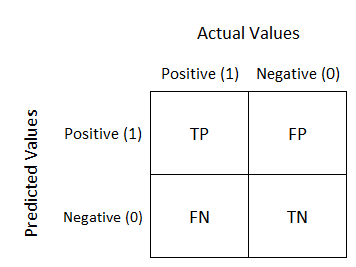
\includegraphics[width=0.6\textwidth]{./img/confusion_matrix}
    \caption{\label{fig:confusion_matrix} Confusion Matrix~\autocite{Jain2020}}
\end{figure}

\section{Hosting}
\subsection{Hosten op lokaal netwerk}
Wanneer er de parameter ``host'' wordt meegegeven aan het programma zelf met als waarde ``0.0.0.0'', dan zal de applicatie opengesteld worden in het lokaal netwerk. De applicatie zal dan draaien op het lokaal IP-adres van de computer of server. Op Windows kan men dit opzoeken door ``ipconfig'' in te typen in \textit{command prompt}. Het IP-adres is dan terug te vinden bij ofwel Ethernet-adapter of WLAN-adapter.

\subsection{Installatie op host}
Om de website te kunnen hosten, moet de nodige software eerst geïnstalleerd worden. Zo kunnen alle Python-bibliotheken geïnstalleerd worden via het volgende commando:
\begin{python}
	pip install -r requirements.txt
\end{python}
Dit commando zorgt er voor dat alle Python-bibliotheken uit dat bestand geïnstalleerd worden zoals het tijdens de \textit{proof-of-concept} geïnstalleerd was.

Daarnaast moet ook FFmpeg apart geïnstalleerd worden. De stappen daarvan staan beschreven op de volgende website: \url{https://www.wikihow.com/Install-FFmpeg-on-Windows} voor een Windows besturingssysteem.

\subsection{SSL-certificaat}
Zodat andere toestellen aan de laptop of server zouden kunnen moet er een SSL-certificaat geïnstalleerd worden. Dit kan bekomen worden door de volgende stappen uit te voeren:
\begin{itemize}
	\item Installeer ``pyopenssl''; voorbeeld via \textit{installer} ``chocolatey''.
	\item ``openssl req -x509 -newkey rsa:4096 -nodes -out cert.pem -keyout key.pem -days 365''
	\item Kopieer ``cert.pem'' en ``key.pem'' naar de plaats van de Flask-applicatie.
	\item Voeg de opties toe:
	\begin{python}
		import ssl
  		context = ssl.SSLContext()
		context.load_cert_chain("cert.pem", "key.pem")
		app.run(ssl_context=context, host='0.0.0.0', ...)
	\end{python}
\end{itemize}

